\chapter{Introduction}
\label{chp:introduction}


Autonomous cars have the potential to revolutionize transportation by providing mobility to a broad range of people. 
These vehicles will (a) increase the independence of those who are incapable of driving, (b) reduce the number of road accidents caused by driver negligence, and (c) reduce both road congestion and pollution by optimising routes and driving style. 
These are just a few ways in which autonomous cars are expected to impact our daily lives \cite{klaver}. 
However, there are numerous challenges to large scale deployment of road-going autonomous cars. 
In particular, public roads are an unpredictable environment, and autonomous cars face a wide variety of scenarios which are difficult to program for.
There are many edge cases which will require the vehicle to not only respond quickly, but also operate at its handling limits to avoid collisions and ensure the safety of its occupants \cite{Barab_s_2017}. 
Autonomous race car development becomes useful in the context of addressing these edge cases.

\section{Research motivation}
The emergence of autonomous racing as a research field stems from the increasing popularity of autonomous vehicles, along with the need to develop driving software robust enough to handle edge cases that require the vehicle to operate at its handling limit.
Racing leagues such as F1tenth \cite{f1tenth} provide a safe and controlled environment for teams to design and improve driving algorithms with a clear evaluation metric in mind: achieving the fastest lap time for navigating around a track \cite{Betz2021}. 
F1tenth achieves this safe and competitive environment by specifying the use of a miniature remote controlled (RC) car chassis as the basis for the vehicle platform. 
The standardised vehicle for the F1tenth racing league is shown in Figure \ref{fig:f1tenth_car}.

\begin{figure}
\centering
  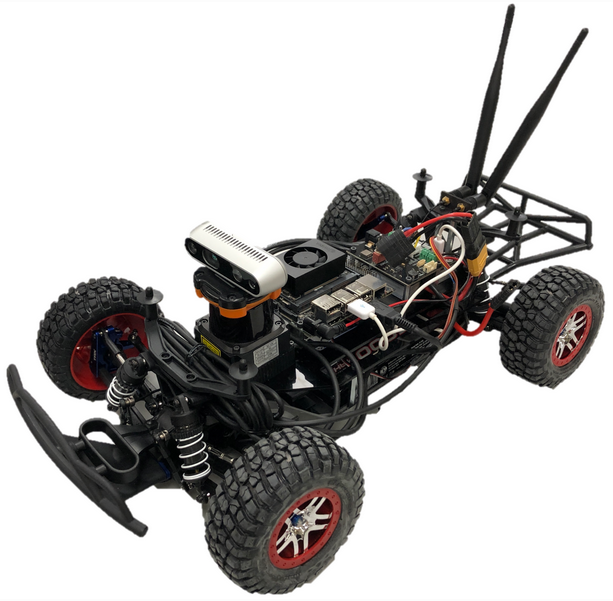
\includegraphics[width=.4\textwidth]{contents/chapt1/figs/f1tenth_car.png}
  \captionof{figure}[The F1tenth standard racecar]{The F1tenth standard vehicle, built on the chassis of a miniature RC car \cite{f1tenth}.}
  \label{fig:f1tenth_car}
\end{figure}

Autonomous racing has led to novel ideas which may directly lead to breakthroughs in the safe production of driverless car technology, especially in those edge cases where cars must operate close to their handling limits to avoid collisions \cite{Weiss2020a}.
This is because racing can be seen as a proxy for the production car edge case, as the major difference between road going and racing cars is the speed of operation \cite{Wadekar2021}.
As such, if a driving algorithm is effective in the extreme racing scenario, then similar design principles can be followed to develop driving algorithms for the road-going case \cite{Weiss2020a}.
However, deploying autonomous race cars does not come without difficulty either.


%\begin{figure}
%\centering
%\begin{minipage}{.5\textwidth}
%  \centering
%  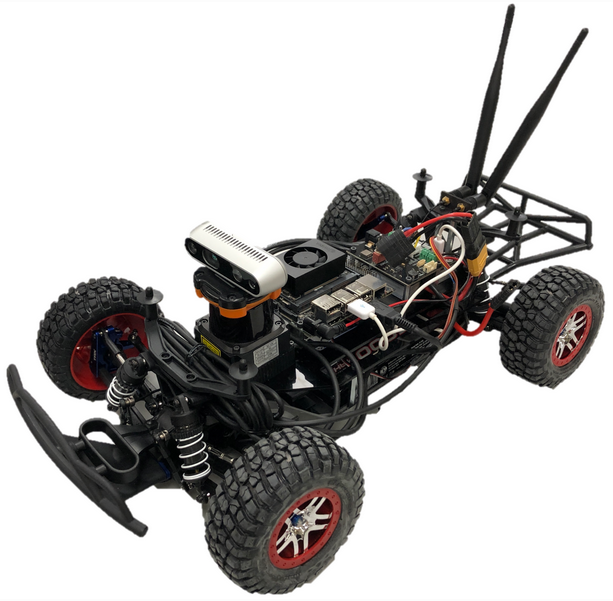
\includegraphics[height=.6\linewidth]{contents/chapt1/figs/f1tenth_car.png}
%  \captionof{figure}[The F1tenth standard racecar]{The F1tenth standard \\racecar.}
%  %[F1tenth standard racecar]{The F1tenth standard racecar}
%  \label{fig:f1tenth_car}
%\end{minipage}%
%\begin{minipage}{.5\textwidth}
%  \centering
%  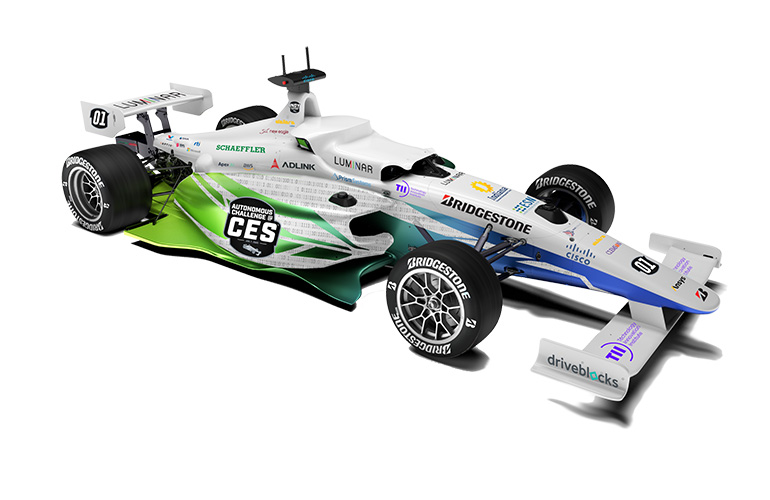
\includegraphics[height=.6\linewidth]{contents/chapt1/figs/indy_auto_car.jpg}
%  \captionof{figure}[The Indy Autonomous challenge official racecar]{Dallara AV-21, the Indy Autonomous challenge official racecar.}
%  %\caption[Indy Autonomous challenge official racecar]{Dallara AV-21, the Indy Autonomous challenge official racecar}
%  \label{fig:iac_car}
%\end{minipage}
%\end{figure}


Deploying autonomous driving algorithms onto physical vehicles presents a major challenge known as the sim2real gap.
This gap exists because driving algorithms rely heavily on an assumed vehicle dynamics models to make decisions.
This vehicle model is only an approximation of the real system dynamics, and discrepancies always exist between the simulated and actual vehicle dynamics due to the difficulty of measuring the parameters of the vehicle precisely \cite{Hewing2018}. 
The tire friction coefficient is a relevant example because it is difficult to characterise the tire-road interaction.
Tire friction varies along the track and is a function of track roughness, tire and track temperature and tire degradation, all of which vary during the race \cite{Sharp2016}.

An inaccurate vehicle model can cause the vehicle to deviate from its intended path which can have catastrophic consequences.
Referring back to the tire friction example, if the actual peak static tire friction is lower than estimated, then there is a risk that the tires will enter into the kinetic friction region.
This will likely result in loss of control of the vehicle.
The issue of model inaccuracy is especially pertinent in the racing case, as racing necessitates that the vehicle travels at high speeds and accelerations, and therefore close to the peak static friction limits of its wheels.
Using this example, we see the importance of designing driving algorithms that are robust to model inaccuracies.
Furthermore, the development of algorithms for racing that are robust to model inaccuracies are expected to benefit production vehicles by providing solutions to handle edge cases where inaccurate models are an issue.

A recent breakthrough in racing algorithm design is the end-to-end pipeline, whereby a neural network is trained to map sensor data directly to control actions.
In particular, reinforcement learning (RL) approaches have shown state of the art results in a variety of scenarios, including time trial and multi-vehicle racing \cite{Fuchs2021, Song2021}.
Reinforcement learning optimises a neural network policy to maximise a scalar reward signal through direct interaction with the environment \cite{Plaat_2022}.
It is a powerful technique that is able to learn non-trivial behaviour from complex cost formulations for systems with non-linear dynamics.  
Furthermore, learning-based systems can leverage real-world data to improve their action policy or vehicle dynamics model.

However promising the results from approaches utilising the end-to-end pipeline are, most applications are still limited to simulation.
There is difficulty in deploying end-to-end systems due to the degradation in performance caused by vehicle model inaccuracies \cite{Ivanov2020}.


Drawbacks - struggles with sim2real

Partial end-to-end


that improve the vehicle dynamics model or action policy with real-world data and allow more complex cost formulations and non-linear dynamics \cite{Fuchs2021}.


Current research in developing autonomous racing software architectures fall into one of three broad categories: the classic, end-to-end, and partial end-to-end approaches.
The classic approach decouples the racing problem into a series of separate modules, namely perception, planning and control \cite{Fuchs2021}.
This is shown in Figure \ref{fig:architecture_comparison} (a). 


Perception algorithms derive knowledge about the vehicles surroundings. 
This includes constructing a map, localising the vehicle, and detecting objects. 
The function of trajectory planning is to compute a minimum time trajectory through this map, consisting of a path ($x$ and $y$ coordinates) and velocity. Controllers then compute actuator commands that minimise the error between the actual and planned trajectory which facilitates the deployment of driving software onto physical vehicles \cite{Betz2021}. 
Classical approaches have achieved impressive results owing to the use of optimisation techniques for planning and control. 
However, there are limitations to these optimisation techniques, such as the requirement for expensive computation (especially for non-linear dynamic models), expensive sensor suites due to the need for frequent and accurate state information, and lack of flexibility in the cost function. 
In particular, reliance on an accurate vehicle dynamics model is a serious issue due to the difficulty of measuring the model parameters \cite{Kabzan2019, Pan2017}.

\begin{figure}[!htb]
\centering
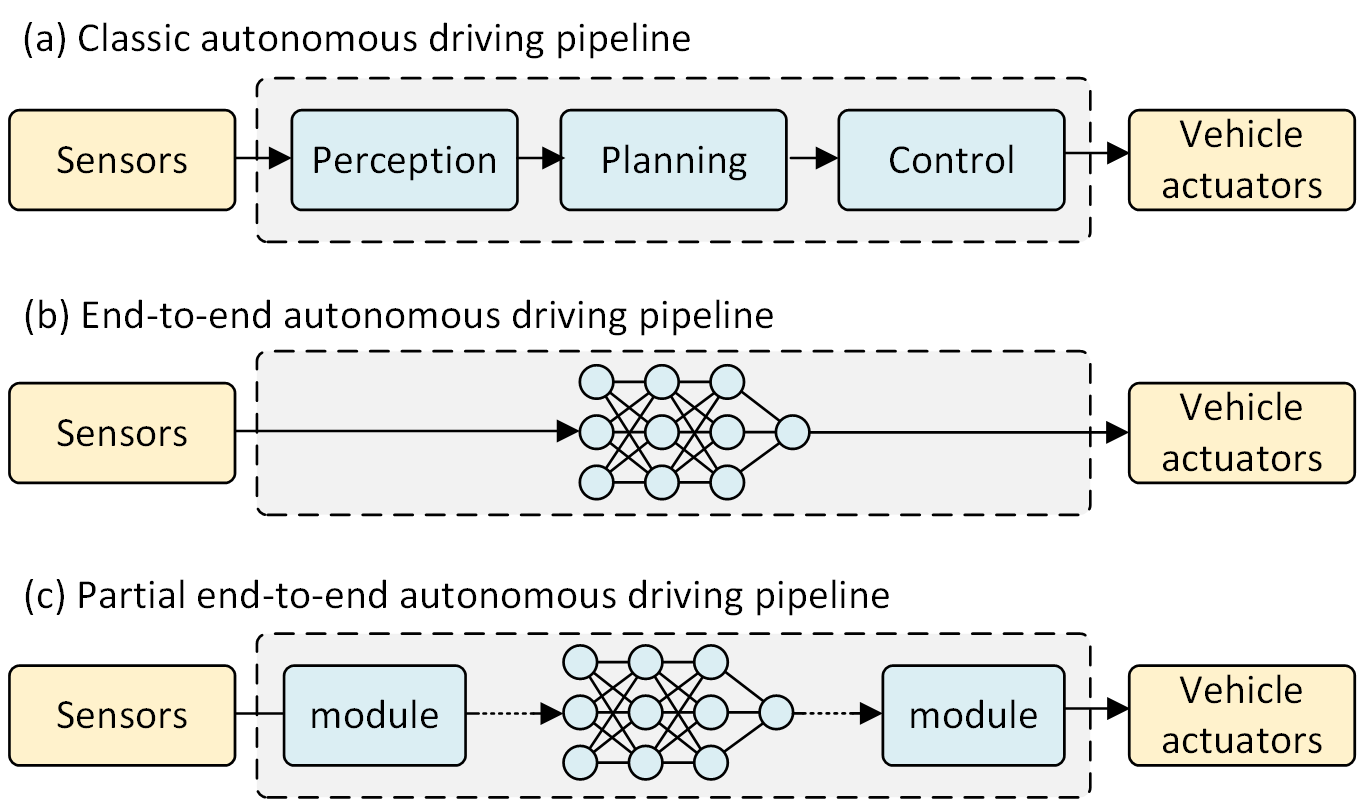
\includegraphics[width=\textwidth*8/10]{contents/chapt1/figs/architecture_comparisons.png}
\caption[A comparison of the commonly used driving software architectures]{A comparison of the commonly used driving software architectures.}
\label{fig:architecture_comparison}
\end{figure}

The limitations of classical methods has led to research in learning-based systems that improve the vehicle dynamics model or action policy with real-world data and allow more complex cost formulations and non-linear dynamics \cite{Fuchs2021}.
Many learning approaches use an end-to-end pipeline, illustrated in Figure \ref{fig:architecture_comparison} (b), whereby a single neural network predicts control outputs from sensor data \cite{Betz2021}.
The neural networks used in end-to-end approaches are typically trained using imitation or reinforcement learning paradigms.
Imitation learned neural networks are trained to mimic an expert such as a human or optimisation method.
This is particularly useful when the neural network has access to lower cost sensors, allowing the optimisation method policy to be executed on a cheaper sensor suit \cite{Pan2017}. 
Neural networks trained with imitation learning have also shown greater robustness to sensor failure and faster online execution time \cite{Wadekar2021} than expert optimisation methods \cite{Lee2019}. 
However, imitation learning is not a suitable method for training a neural network policy in scenarios where expert training data is not available, as in cases where optimisation methods fail \cite{Fuchs2021a}.

%Reinforcement learning
Reinforcement learning optimises a neural network policy to maximise a scalar reward signal through direct interaction with the environment \cite{Plaat_2022}. 
The benefit of using reinforcement learned neural networks are similar to the imitation learning approach, i.e., less stringent sensor requirements, robustness to sensor failure, and fast online execution time. However, the technique allows for more complex cost formulation and negates the need for expert training data \cite{Fuchs2021}.
The approach has shown state of the art results in both time trail and multi-agent settings \cite{Song2021}.
However promising the results from approaches utilising the end-to-end pipeline are, most applications are still limited to simulation.
There is difficulty in deploying end-to-end systems due to the degradation in performance caused by vehicle model inaccuracies \cite{Ivanov2020}, as discussed in Section \ref{sec:auto_race_challenges}. 
These difficulties are usually overcome by retraining the neural network policy on the physical vehicle after deployment, which is an inherently risky process, as retraining the policy network requires exploration which may result in the vehicle crashing \cite{Chisari2021}.
Furthermore, neural network behaviour is difficult to interpret, especially where the neural network takes the place of the entire driving pipeline \cite{Evans2021}.


A relatively unexplored possibility to address issues from the end-to-end approach is to synthesise the classic and end-to-end pipelines by modifying a section of the classic pipeline with a neural network, as shown in Figure \ref{fig:architecture_comparison}. 
This is known as a partial end-to-end pipeline \cite{Betz2021}. 
In particular, a promising approach to address the degradation in performance of end-to-end systems due to model inaccuracies is to use a neural network for trajectory prediction, in conjunction with a set of controllers for trajectory tracking \cite{Capo2020}.
This approach benefits from the advantages of learning-based end-to-end systems, i.e., complex cost formulation, fast online computation and learning from real-world data, while also leveraging the reliability of the hierarchical structure from the classical approach \cite{Ghignone2022}. 


\section{Project objectives and scope}
\label{sec:objectives}

Our goal is to investigate and develop a partial end-to-end driving autonomous driving software architecture as a method to address issues with typical learning, i.e. end-to-end approaches, with specific reference to robustness to inaccuracies in the vehicle model. Therefore, the objective of the project is two-fold:

\begin{enumerate}
  \item Develop a framework for partial end-to-end autonomous racing software
  \item Benchmark the partial end-to-end framework against end-to-end techniques with and without model discrepancies
\end{enumerate}

We do so within a simulated F1Tenth racing simulation environment. 
This platform is easily extended to real-world vehicles, allowing for the easy extension of future work on the topic.
The autonomous driving software is developed to achieve the goals of navigating the vehicle around the track while minimising lap time and number of collisions. 
The exact scenario we solve for is a time trial, whereby there is only one vehicle on the track at a time. Furthermore, we make the assumption that the track dimensions are perfectly known. 
Finally, we choose to limit the scope of the project by only developing reinforcement learning techniques for training to negate the requirement for expert training data.


\section{Document outline}
\label{sec:outline}

Chapter \ref{chp:litreview} constitutes an overview of the existing approaches to solving the autonomous racing problem in literature. 
We briefly discuss solutions from the classic pipeline and end-to-end pipelines, before reviewing partial end-to-end approaches. 
The core concepts of Markov decision processes reinforcement learning are then discussed in Chapter \ref{chp:reinforcement_learning}.
This is followed by a description of the simulation setup for the racing environment in Chapter \ref{chp:simulation}.
Our partial end-to-end system design is detailed in Chapter \ref{chp:design}, followed by experiments and results in Chapter \ref{chp:experiments}. 
We conclude with a summary of our findings and proposal for future work in Chapter \ref{chp:conclusion}.

